%
% FH Technikum Wien
% !TEX encoding = UTF-8 Unicode
%
% Erstellung von Master- und Bachelorarbeiten an der FH Technikum Wien mit Hilfe von LaTeX und der Klasse TWBOOK
%
% Um ein eigenes Dokument zu erstellen, müssen Sie folgendes ergänzen:
% 1) Mit \documentclass[..] einstellen: Master- oder Bachelorarbeit, Studiengang und Sprache
% 2) Mit \newcommand{\FHTWCitationType}.. Zitierstandard festlegen (wird in der Regel vom Studiengang vorgegeben - bitte erfragen)
% 3) Deckblatt, Kurzfassung, etc. ausfüllen
% 4) und die Arbeit schreiben (die verwendeten Literaturquellen in Literatur.bib eintragen)
%
% Getestet mit TeXstudio mit Zeichenkodierung ISO-8859-1 (=ansinew/latin1) und MikTex unter Windows
% Zu beachten ist, dass die Kodierung der Datei mit der Kodierung des paketes inputenc zusammen passt!
% Die Kodierung der Datei twbook.cls MUSS ANSI betragen!
% Bei der Verwendung von UTF8 muss dnicht nur die Kodierung des Dokuments auf UTF8 gestellt sein, sondern auch die des BibTex-Files!
%
% Bugreports und Feedback bitte per E-Mail an latex@technikum-wien.at
%
% Versionen
% *) V0.7: 9.1.2015, RO: Modeline angepasst und verschoben
% *) V0.6: 10.10.2014, RO: Weitere Anpassung an die UK
% *) V0.5: 8.8.2014, WK: Literaturquellen überarbeitet und angepasst
% *) V0.4: 4.8.2014, WK: Initalversion in SVN eingespielt
%
\documentclass[Bachelor,BIF,english]{twbook}
\usepackage[utf8]{inputenc}
\usepackage[T1]{fontenc}

%
% Bitte in der folgenden Zeile den Zitierstandard festlegen
\newcommand{\FHTWCitationType}{IEEE} % IEEE oder HARVARD möglich - wenn Sie zwischen IEEE und HARVARD wechseln, bitte die temorären Dateien (aux, bbl, ...) löschen
%
\ifthenelse{\equal{\FHTWCitationType}{HARVARD}}{\usepackage{harvard}}{\usepackage{bibgerm}}

% Definition Code-Listings Formatierung:
\usepackage[final]{listings}
\lstset{captionpos=b, numberbychapter=false,caption=\lstname,frame=single, numbers=left, stepnumber=1, numbersep=2pt, xleftmargin=15pt, framexleftmargin=15pt, numberstyle=\tiny, tabsize=3, columns=fixed, basicstyle={\fontfamily{pcr}\selectfont\footnotesize}, keywordstyle=\bfseries, commentstyle={\color[gray]{0.33}\itshape}, stringstyle=\color[gray]{0.25}, breaklines, breakatwhitespace, breakautoindent}
\lstloadlanguages{[ANSI]C, C++, [gnu]make, gnuplot, Matlab}

%Formatieren des Quellcodeverzeichnisses
\makeatletter
% Setzen der Bezeichnungen für das Quellcodeverzeichnis/Abkürzungsverzeichnis in Abhängigkeit von der eingestellten Sprache
\providecommand\listacroname{}
\@ifclasswith{twbook}{english}
{%
    \renewcommand\lstlistingname{Code}
    \renewcommand\lstlistlistingname{List of Code}
    \renewcommand\listacroname{List of Abbreviations}
}{%
    \renewcommand\lstlistingname{Quellcode}
    \renewcommand\lstlistlistingname{Quellcodeverzeichnis}
    \renewcommand\listacroname{Abkürzungsverzeichnis}
}
% Wenn die Option listof=entryprefix gewählt wurde, Definition des Entyprefixes für das Quellcodeverzeichnis. Definition des Macros listoflolentryname analog zu listoflofentryname und listoflotentryname der KOMA-Klasse
\@ifclasswith{scrbook}{listof=entryprefix}
{%
    \newcommand\listoflolentryname\lstlistingname
}{%
}
\makeatother
\newcommand{\listofcode}{\phantomsection\lstlistoflistings}

% Die nachfolgenden Pakete stellen sonst nicht benötigte Features zur Verfügung
\usepackage{blindtext}
\usepackage{parskip}
\usepackage{epstopdf}
\usepackage{url}
\usepackage{breakurl}

%
% Einträge für Deckblatt, Kurzfassung, etc.
%
\title{Rebuilding a SharePoint 2013 Application with Angular 7 and Reactive Programming}
\author{Dominik Hack}
\studentnumber{1610257044}
\supervisor{DI Thomas Rongitsch}
\place{Vienna}
\kurzfassung{text}
\schlagworte{schlagwort1}
\outline{text}
\keywords{keyword1}

\begin{document}

%Festlegungen für den HARVARD-Zitierstandard
\ifthenelse{\equal{\FHTWCitationType}{HARVARD}}{
\bibliographystyle{Harvard_FHTW_MR}%Zitierstandard FH Technikum Wien, Studiengang Mechatronik/Robotik, Version 1.2e
\citationstyle{dcu}%Correct citation-style (Harvardand, ";" between citations, "," between author and year)
\citationmode{abbr}%use "et al." with first citation
\iflanguage{ngerman}{
    %Deutsch Neue Rechtschreibung
    \newcommand{\citepic}[1]{(Quelle: \protect\cite{#1})}%Zitat: Bild
    \newcommand{\citefig}[2]{(Quelle: \protect\cite{#1}, S. #2)}%Zitat: Bild aus Dokument
    \newcommand{\citefigm}[2]{(Quelle: modifiziert "ubernommen aus \protect\cite{#1}, S. #2)}%Zitat: modifiziertes Bild aus Dokument
    \newcommand{\citep}{\citeasnoun}%In-Line Zitiat entweder mit \citep{} oder \citeasnoun{}
    \newcommand{\acessedthrough}{Verf{\"u}gbar unter:}%Für URL-Angabe
    \newcommand{\acessedthroughp}{Verf{\"u}gbar bei:}%Für URL-Angabe (Geschützte Datenbank, Zugriff durch FH)
    \newcommand{\acessedat}{Zugang am}%Für URL-Datum-Angabe
    \newcommand{\singlepage}{S.}%Für Seitenangabe (einzelne Seite)
    \newcommand{\multiplepages}{S.}%Für Seitenangabe (mehrere Seiten)
    \newcommand{\chapternr}{K.}%Für Kapitelangabe
    \renewcommand{\harvardand}{\&}%Harvardand in Zitaten
    \newcommand{\abstractonly}{ausschließlich Abstract}
    \newcommand{\edition}{. Auflage}%Angabe der Auflage
}{
\iflanguage{german}{
    %Deutsch
    \newcommand{\citepic}[1]{(Quelle: \protect\cite{#1})}%Zitat: Bild
    \newcommand{\citefig}[2]{(Quelle: \protect\cite{#1}, S. #2)}%Zitat: Bild aus Dokument
    \newcommand{\citefigm}[2]{(Quelle: modifiziert "ubernommen aus \protect\cite{#1}, S. #2)}%Zitat: modifiziertes Bild aus Dokument
    \newcommand{\citep}{\citeasnoun}%In-Line Zitiat entweder mit \citep{} oder \citeasnoun{}
    \newcommand{\acessedthrough}{Verf{\"u}gbar unter:}%Für URL-Angabe
    \newcommand{\acessedthroughp}{Verf{\"u}gbar bei:}%Für URL-Angabe (Geschützte Datenbank, Zugriff durch FH)
    \newcommand{\acessedat}{Zugang am}%Für URL-Datum-Angabe
    \newcommand{\singlepage}{S.}%Für Seitenangabe (einzelne Seite)
    \newcommand{\multiplepages}{S.}%Für Seitenangabe (mehrere Seiten)
    \newcommand{\chapternr}{K.}%Für Kapitelangabe
    \renewcommand{\harvardand}{\&}%Harvardand in Zitaten
    \newcommand{\abstractonly}{ausschließlich Abstract}
    \newcommand{\edition}{. Auflage}%Angabe der Auflage
}{
    %Englisch
    \newcommand{\citepic}[1]{(Source: \protect\cite{#1})}%Zitat: Bild
    \newcommand{\citefig}[2]{(Source: \protect\cite{#1}, p. #2)}%Zitat: Bild aus Dokument
    \newcommand{\citefigm}[2]{(Source: taken with modification from \protect\cite{#1}, p. #2)}%Zitat: modifiziertes Bild aus Dokument
    \newcommand{\citep}{\citeasnoun}%In-Line Zitiat entweder mit \citep{} oder \citeasnoun{}
    \newcommand{\acessedthrough}{Available at:}%Für URL-Angabe
    \newcommand{\acessedthroughp}{Available through:}%Für URL-Angabe (Geschützte Datenbank, Zugriff durch FH)
    \newcommand{\acessedat}{Accessed}%Für URL-Datum-Angabe
    \newcommand{\singlepage}{p.}%Für Seitenangabe (einzelne Seite)
    \newcommand{\multiplepages}{pp.}%Für Seitenangabe (mehrere Seiten)
    \newcommand{\chapternr}{Ch.}%Für Kapitelangabe
    \renewcommand{\harvardand}{\&}%Harvardand in Zitaten
    \newcommand{\abstractonly}{Abstract only}
    \newcommand{\edition}{~edition}%Edition -> note, that you have to write "edition = {2nd},"!
}}}

\maketitle
\chapter{Introduction}
SharePoint \cite{SharePoint} is an application developed by Microsoft that supports team collaboration by sharing information, accessible through a browser, in the form of files and sites on specific topics in an intranet. SharePoint Server 2013 is one of several versions of SharePoint. Currently, the latest Version is SharePoint Server 2019 \cite{SharePoint}. One of the reasons why more than 200,000 organizations worldwide utilize SharePoint is the ability to customize each tool, library, and control it consist of \cite{SharePoint} \cite{SharePointDevRef}.
\\[\baselineskip]
This work is part of a company project to extend the SharePoint Blog feature. The extension of this feature was ordered by a customer whose company uses SharePoint Server 2013 as a solution for their intranet. This SharePoint was configured in 2015 as part of a project commissioned by the customer. Some of the default features of SharePoint were adapted to the customer's needs, and new features were developed as well. Over time, individual features have been modified and new ones have been added. However, none of the other changes have been as extensive as the requirements for the new blog feature. The following were the demanded features: 
\begin{itemize}
\item The design of the default blog site should be redesigned.
\item Blog posts should be able to be labeled with tags. 
\item Filtering of blog entries depending on categories and tags should be added.
\item User should be able to subscribe to tags and categories. 
\item The role alert manager should be added.
\item An alert manager should be able to subscribe other users to tags or categories.
\item The automatically generated sidebar from SharePoint should be hidden. 
\item Pagination should be added.
\item Pagination should be configurable for each blog site.
\item Features should be hidden or displayed depending on user rights.
\end{itemize}

According to an estimate of the cost of all features, the three-person development team would be busy working on this project for several weeks. However, instead of continuing to build on the legacy SharePoint project, the idea was to rebuild the default SharePoint blog feature with the desired extensions in Angular with the latest state of the art practices and then integrate the application in SharePoint. One reason why this approach was chosen was that the estimated effort of such an Angular application stayed within reason of the ordered project. Another reason was that extending the functionality of SharePoint's default features sometimes had to be resolved by injecting JavaScript code, which leads to a chaotic project structure. The last reason was that only one developer of the company knew how to find all the necessary files to maintain the old SharePoint project properly.
\\[\baselineskip]
This thesis aims to describe the development phase of this project. Thereby, the best practice methods employed in organizing the project, planning the software architecture and developing the application will be discussed. In addition, the effectiveness of quality assurance through repetitive processes such as code reviews, pull requests, and Test Driven Development will be addressed. All of the methods mentioned above were adopted in the development of this application because the goal was to develop software that could be extended much more straightforward with new features and needed less effort and time to maintain than the old SharePoint project.
\\[\baselineskip]
Therefore the following research questions are the focus of this work:
\begin{itemize}
\item Which changes have to be made in the project so that the application or already existing components can be extended in functionality?
\item Is the blog feature more maintainable because it was implemented in a new project instead of the old SharePoint project?
\end{itemize}

\clearpage


\chapter{Tools \& Frameworks} 
what will be presented in this chapter (reactive programming; tools to use this paradigm with: ReactiveX, Redux and NgRx; Angular; why typescript; what components are; introduction of important tools used by angular: npm, webpack and babel),
For the implementation of this project a technology had to be decided on that meets the requirements of being integrated into and communicate with SharePoint 2013.

\section{Reactive Programming}
If an interaction with a reactive application takes place, a event occurs which the software will respond on by reacting on it in a certain way. Therefore a reactive software system could be any application with a graphical user interface (GUI) reacting on user input, a network monitoring service reacting on certain changes of the network or even a simple calculator reacting on button presses. reactive applications can become complex because of a mixed combination of data and control flow \cite[p.~1]{PositivEffectOfRP}, 
two main approaches to implement a reactive application (also explain figure):
\begin{figure}[!htbp]
\centering
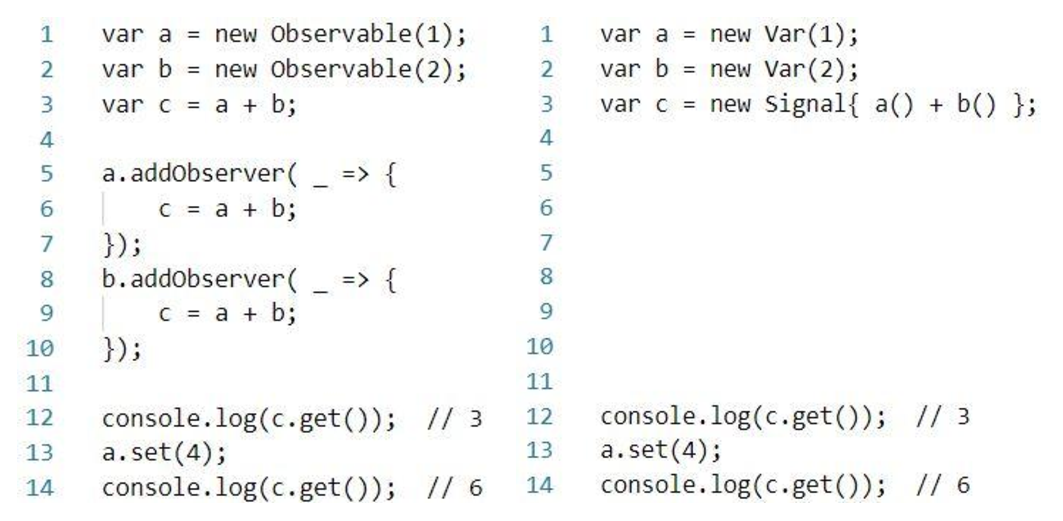
\includegraphics[width=0.75\linewidth]{PICs/pseudo_Code_reactive_2_ways.eps}
\caption{JavaScript-like pseudo code of the observer pattern approach (left) and the signals and vars approach (right) \cite[p.~797]{DebuggingRP} \cite[p.~3]{PositivEffectOfRP}}\label{Fig1}
\end{figure}
traditional approach observer pattern \cite[p.~360-372]{ObserverDP}, decouples event consumers from event producers \cite[p.~953]{RPWalkthrough}, (in object oriented programming using observer pattern, decouples observers or subscribers from observables or subjects, observers subscribe to observables, observables do not know their subscribers, when observables change their state they notify their observers depending on the implementation this can be done through emitting events. When a subscriber learns of a change in the state of the subject, he adjusts his state to that of the subject. \cite[p.~363]{ObserverDP}),
vs the other way, what is reactive programming: programming paradigm supporting language-level abstractions \cite[p.~953]{RPWalkthrough}, The four principles all implementations of reactive programming pursue are:
\begin{itemize}
\item Declarativeness: declaring how the states of the components depend on each other, not how to retrieve the state when changes occur \cite[p.~2]{PositivEffectOfRP}.
\item Abstraction over change propagation: No need to manually update dependencies, propagation of change is handled by language runtime \cite[p.~2]{PositivEffectOfRP}.
\item Composability: Composing reactive computations through abstractions \cite[p.~2]{PositivEffectOfRP}.
\item Favoring data flow over control flow: Calculations of the software system are triggered by new data or events and are not depending on the execution of the control flow \cite[p.~2]{PositivEffectOfRP}.
\end{itemize}
einiges an Forschung wurde schon betrieben und nach der Einführung von funcitonal reactive programming in Haskell wurde dieses konzept auch in Scheme (FrTime \cite{FrTime}), Scala (Scala.react \cite{DeprecatingOP}) und JavaScript (Flapjax \cite{Flapjax}) implementiert, sogar wurde in Microsofts Reactive Extensions (RX or ReactiveX) konzepte von reactive programming implementiert \cite[p.~954]{RPWalkthrough} \cite[p.~796]{DebuggingRP} \cite[p.~2]{PositivEffectOfRP}
(signals or behaviours: time changing values, treated as constraints of the language runtime, when an inconcistency of a signal or behaviour is detected a recalculation is triggered \cite[p.~797]{DebuggingRP} \cite[p.~3]{PositivEffectOfRP}, can either depend on other signals or vars, vars are reactive values like signals but without dependencies \cite[p.~2]{PositivEffectOfRP}), less error prone, easier to understand, still immature field -> lack of developer tools like debuggers \cite[p.~796]{DebuggingRP}

\subsection{ReactiveX}
general introduction (what is it \cite{ReactiveExtensions} \cite[p.~291]{RxAngular5Prj} (von Microsoft aber open source), why should it be used) \cite{ReactiveX}, bringing functional-reactive-programming-like reactivity (FRP-like reactivity \cite{PositivEffectOfRP}
marble-diagrams
\begin{figure}[!htbp]
\centering
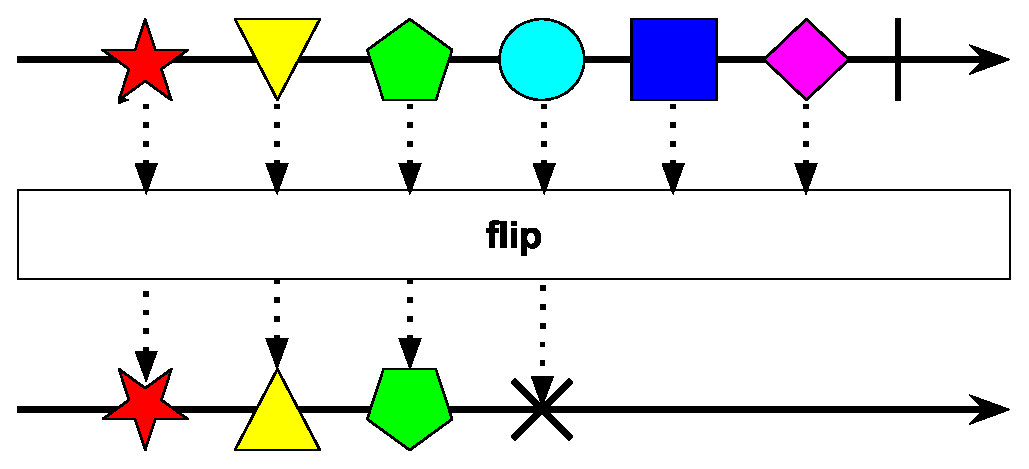
\includegraphics[width=0.5\linewidth]{PICs/marble_diagram.eps}
\caption{An example of a marble diagram, which is mostly used for explaining transformations of observables \cite{RxObservables}.}\label{Fig2}
\end{figure}
observables, observables background with reactor pattern \cite{RxObservables} \cite[p.~292]{RxAngular5Prj} \cite[p.~310]{RxAngular5Prj}
hot and cold \cite{RxObservables}

\subsection{Redux}
general introduction (what is it, why should it be used), \cite{Redux}, motivation why redux \cite{ReduxIntroMoti}, core concept \cite{ReduxIntroCC}, three principles \cite{ReduxIntro3P}, figure for explanation

\subsection{NgRx}
general introduction (what is it, why should it be used), \cite{Ngrx}, ng/store, effects


\section{Angular}
what is angular? what is it for? \cite[p.~xxiv-xxix]{RxAngular5Prj}, dependency injection \cite[p.~]{YakovFainAngular} \cite[p.~211]{RxAngular5Prj}, data binding, \cite[p.~]{YakovFainAngular}, bundeling code in modules \cite[p.~116]{RxAngular5Prj}
polyfills \cite[p.~18]{RxAngular5Prj}

\subsection{TypeScript}
general introduction \cite[p.~19]{RxAngular5Prj} \cite{TypeScript} \cite[p.~41]{RxAngular5Prj} (what is it, why should it be used),

\subsection{Components}
general introduction \cite[p.~22]{RxAngular5Prj} \cite[p.~89]{RxAngular5Prj} \cite[p.~159]{RxAngular5Prj} (what is it, why should it be used, structured inside of a module), 

\subsection{npm}
general introduction \cite[p.~71]{RxAngular5Prj} (what is it, why should it be used), 
tool to install everything js based

\clearpage 

\chapter{Implementation}
The following sections deal with describing the processes utilized to ensure the quality of the final product both during the development phase and after completion. First, the general procedures related to project management and continuous integration are illustrated. Subsequently, the software architecture including the project structure, the interfaces and additionally added technologies as well as methodologies will be presented. Finally, the development with reactive programming is discussed.

\section{Project Management}
To successfully complete this project with as few errors as possible and to develop a product that adds business value to the customer and satisfies the customers' needs, the agile project management framework "Scrum" \cite{Scrum} was employed. 
\\[\baselineskip]
The scrum team consisted of three developers, one of whom was one half of his time involved in scrum master activities, and one product owner. The product owner took care of analyzing the current problems together with the customer in order to develop a possible solution. Based on these requirements, a first version of the backlog was created to give the development team an overview of the product to be developed. Subsequently, the developer team estimated the story points of each user story using planning poker. With this information the product owner calculated the offer for the customer. After the contract was signed the scrum team met for a project kick-off meeting to discuss the highest priority user stories and refine the backlog for the first sprint.
\\[\baselineskip]
The length of a sprint for this project was one week, since at first the user stories were small enough so that the commitment to the sprint goal could be kept. Later, the length of a sprint was increased to two weeks, because on the one hand some user stories were too large to finish in a week and on the other hand a developer had to be assigned to other projects for some time. Sprints were planned using the user-story- and task-board-backlog tools provided by the company's TFS (Team Foundation Server) \cite{TFS}. After each sprint a short retro was held on the day of the planning where the finished user stories and the problems encountered while implementing them were deliberated. In addition when it occurred that a commitment could not be kept, the reasons were sought to make adjustments to user stories that could be affected. 
\\[\baselineskip]
Every day a daily stand-up was held where each developer announced the current status of their to them assigned user stories. If there was any difficulty implementing a user story, after the meeting, the task in question was discussed with at least one other developer. If no solution was found, the product owner was contacted to discuss the problem. This led in most cases to an adaptation of the acceptance criteria of the user story, only rarely the customer had to be contacted to discuss the respective requirement. 
\\[\baselineskip]
If all tasks of a user story were implemented and thus also fulfilled all acceptance criteria, the user story could be closed and a pull request could be created. The pull request was accepted when another developer agreed to the changes and the build process, which is described in more detail in the next chapter, succeeded. So that a user story was now considered as resolved, the product owner together with the developer tested the respective features on the development server. If changes still had to be made, the user story was set to active as long as there was still enough time in the running sprint otherwise it was put back in the backlog to be scheduled for the next sprint. After a certain number of user stories were resolved, a milestone was reached, meaning that a demo meeting with the customer was arranged in order to present the current status of the product. As a result, the current application was deployed on the user acceptance test server and then an in-house demo meeting with the scrum team was held to prepare and practice for the upcoming demo meeting with the customer. The feedback given by the customer during the demo meeting was collected by the product owner, who then adjusted the remaining user stories accordingly. If necessary, new user stories were created and added to the backlog. When all the user stories were resolved, a final demo meeting was held with the client, and after the final adjustments were integrated, the product was deployed to the client's production systems.

\section{Continuous Integration}
In order to detect as many bugs as possible before merging the changes with the master branch of the git \cite{Git} repository and maximizing the quality of the source code as well as the project structure, the development team defined a CI process with specific rules for the project. These rules applied to handling the local cloned git repository and when changes to the source code were accepted for merging with the shared repository. 
\\[\baselineskip]
Before starting the implementation of a user story, a feature branch had to be created, because committing on the master branch was not possible due to constraints and after merging the changes into the master branch, the respective branch had to be deleted. If the acceptance criteria of the user story were met, all changes to the source code had to be pushed to the shared repository and a pull request had to be created using the TFS user interface. The pull request was accepted if at least one other developer agreed, no comments on the source code were still marked as active, and the, on creation of the pull request automatically triggered, build process was successfully completed. The review of the source code of the pull request was carried out by a code review with at least one other developer. If changes had to be made to the code after the code review, the pull request remained open. Only when all conditions were fulfilled the pull request was completed.
\\[\baselineskip]
The build pipeline was designed utilizing the build definition user interface of the TFS \cite{TFSBuildPipeline} . The requirements for a build server for this procedure are that it has npm installed and has enough space to download and install the node modules. The build process consists of six tasks which are the following:
\begin{itemize}
\item "Get sources": As the name implies, this build step is responsible for getting the latest source code. When configuring the task, the name of the project, the name of the code repository as well as the name of the branch that should be fetched, after the process started, had to be defined.
\item "npm install": This step executes the command "npm install" and thus installs all required dependencies of the application which are defined in the "package-lock.json" file \cite{NpmInstall}. In the configuration of the step, the folder in which the "package.json" is located was specified, as this allows the task to keep in mind the additional configurations for the particular command to be executed \cite{NpmTaskInstall}.
\item "npm build": The use of this step is it to start a production build process. A custom command must be specified for this step because the build definition tool of the companies TFS did not support the command "npm run build" out of the box and furthermore additional arguments for the command had to be specified. The command that is executed is "npm run prod-build" which is an abbreviation for "ng build --prod --output-path='dist/blog-app'" defined in the "package.json" file. The argument "--prod" sets the production-flag to true and thereby executes a build which does not only employ bundeling and limited tree-shaking but also limited dead code elimination. The argument "--output-path" specifies the relative path to the folder where the compiled project will be moved \cite{AngularCliBuild}. As with the previous step, the folder in which the "package.json" file is located was specified \cite{NpmTaskCustom}.
\item "npm test": In this step, the test process is initiated. For the same reason as with the "npm build" step a custom command has to be configured. The command specified here is "npm run test-headless" which in turn is a short for "ng test --watch=false --browsers=PhantomJS --reporters=progress,junit". The argument "--watch=false" ensures that the test process is terminated after a run. The other two arguments define which reporter or browser should be operated by karma \cite{KarmaConfig}. As a reporter Progress and JUnit \cite{JUnit} \cite{KarmaJUnitReporter} were chosen, because firstly the test results generated by the Progress reporter can be found in the console output of the build job in the TFS and secondly a more pleasant view of the test results is generated by the TFS in the next step by interpreting the XML output of the test results created by the JUnit reporter. The reason why PhantomJS \cite{PhantomJS} was chosen as the browser in which the tests are running will be explained in the next paragraphs. As with the other two steps before, the folder in which the "package.json" file is was specified again \cite{NpmTaskCustom}.
\item "Publish Test Results": The test results created by the previous task are captured by this task and passed to the TFS in the correct format. The configuration of this build step consists of the respective format of the test results, the name of the file in which the test results are to be found and in which folder this file should be searched for. The name of the output file of the JUnit reporter is, unless the default configuration inside of the karma configuration file is changed, in the pattern "TESTS-Name-Of-Browser{\_}Version-Of-Browser{\_}(Name-Of-Operating-System{\_}Version-Of-Operating-System).xml", therefore "TESTS-*.xml", where "*" serves as a wildcard, was set \cite{KarmaJUnitReporterConfig}. The default value "\$(System.DefaultWorkingDirectory)" for the search folder was retained because no changes were made to the configuration of the output folder of the JUnit Reporter \cite{TFSPublishBuildArtifact}.
\item "Publish Artifact: dist": In the last step, the files created by the build task are issued as artifacts. For this, the path to the folder containing the compiled files and the name of the artifact had to be specified. The value for the path was the output folder specified in the "--output-path" argument of the "npm build" command. For the name of the artifact "drop" was selected because it was a rule of the development team for this project to call each build artifact "drop". An artifact created by this task could be downloaded to manually deploy on a SharePoint 2013 development server or User Acceptance Test Server for further testing by a developer, the product owner or the customer \cite{TFSPublishBuildArtifact}.
\end{itemize}
For this project, the first build process for an Angular project of the development team has been created, which in addition to building the application also runs the tests and then publishes the results. This was mostly because the build servers had problems launching a browser like Google Chrome \cite{Chrome} or Mozilla Firefox \cite{Firefox} however, a browser is needed to run the tests with Karma as the test runner. The solution to this problem was to use a headless browser \cite[p.~2]{HeadlessBrowser} for executing the tests. In contrast to browsers like Google Chrome or Mozilla Firefox, headless browsers are always executed in the background and do not have a graphical user interface. The communication with a headless browser thus only takes place via the console, which allows a build server to run it. The selected headless browser for this project was PhantomJS \cite{PhantomJS}, as two developers of the team had already gained experience with PhantomJS.
\\[\baselineskip]
\begin{figure}[!htbp]
\centering
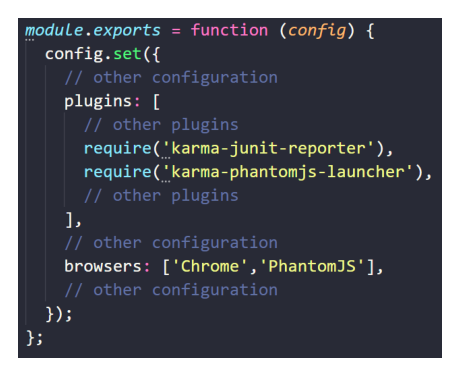
\includegraphics[width=0.5\linewidth]{PICs/karma_phantomjs.eps}
\caption{The "karma.conf.json" file with the configuration to utilize PhantomJS added to it}\label{Fig3}
\end{figure}

For PhantomJS to be operated as a browser for the test task, the three npm packages: phantomjs-prebuilt, karma-phantomjs-launcher, and karma-junit-reporter had to be included in the project and added to the karma configuration file as shown in the figure \ref{Fig3}. These packages install PhantomJs and two karma plugins, which allows Karma to run the tests inside of PhantomJS and create reports of the results which the TFS user interface can interpret and showcase. Additionally, a process variable with the value "C:/NPM/Modules/PhantomJS.cmd" had to be added to the build process, so that the respective agent finds the executable file of PhantomJS.


\section{Integrating Angular in SharePoint 2013}
In order to use Angular as the framework for developing the application, it was first necessary to find a way to host the application in SharePoint 2013. This problem was solved by injecting the compiled project files each inside of one HTML script tag into the script editor web part of the landing page. For the value of the HTML script tag's source attribute the path to the compiled files and for the value of the type attribute "text/javascript" was defined. As a result, when the page was loaded, the scripts were executed and thereby started the application. An advantage of this solution was that every developer could work locally on the blog application because the path to the compiled project files could also point to the output of the build process of the local server hosted by the Angular "ng serve"-command.
\\[\baselineskip]
However, one requirement of the development team was not having to think about the script editor web part of the blog application every time the project was released, which is why it was decided to develop a SharePoint feature \cite{SPFeature} and feature event receiver \cite{SPFeatureEventReceiver}. Furthermore a feature event receiver also solved the question how the data of the old blog application could be migrated automatically.
\\[\baselineskip]
A SharePoint feature, as the name suggests, offers further functionality and can be activated at any time by a user with high enough privileges. A feature event receiver waits until a feature related event shows up to respond to it. Such an event appears when activating, deactivating, installing or deleting a feature. One limitation that has been set up so that elements of the blog feature are not unnecessarily created on the entire system is that the developed feature can only be activated on pages where blogs have already been created. By activating the blog feature, the blog event receiver ensures the creation of all necessary elements and migrates the data from the old blog. The tasks of the blog event receiver are the following:
\begin{itemize}
\item "MigrateBlog": Checks if an old blog is present and if so, the list of blogs and comments is copied to set the respective lists of the new blog application.
\item "EnsurePageLib": Checks the existence of a SharePoint document library \cite{SPDocumentLibrary} on the page of the blog application, if it is not present, one is created. A document library manages files that can be shared among multiple users.
\item "EnsureLandingPage": Checks by means of a configuration file if all necessary web parts of the page have been created, if not they will be created. This ensures the creation of the script editor web part and thereby configures the paths to the compiled project files. In addition, the welcome page in the root folder is set to "Beitraege.aspx".
\item "EnsureCategoryListFields": Ask if a list of categories already exists otherwise a new one will be created. If a list already exists, an additional lookup field is defined and added as this is required for filtering the categories.
\item "EnsureTagsList": Only ensures the creation of a list of tags.
\item "EnsureBlogListFields": Checks if a list has been created for blogs, if not a list will be created. The default blog list will be expanded with fields as they are needed for the new functionality. These include tags, target audiences, content owners, and the time how long a blog post is in the global news section of the SharePoint.
\item "EnsureCategoryItemEventReceiver": Checks the creation of the category item event receiver, if none exists one will be created and configured. This event receiver then ensures that when creating, updating or deleting a category, the category list of alerts is also taken into account.
\item "EnsureTagsItemEventReceiver": Similar to above only this is the event receiver of the tag items.
\item "ReorderFields": This adjusts the default arrangement of the fields in the blog list. The order of the fields not only plays a role when displaying the list but also when creating a new blog. This arrangement was a requirement of the customer.
\item "EnsureAlertManagerGroup": Checks if an alert manager group has been created, if none exist, on will be created. An alert manager has the rights to subscribe to a blog, categories or tags on behalf of others.
\end{itemize}

So that all functionalities of the SharePoint can be used the website must be started in an Internet Explorer \cite{IE}. Since this browser does not support all the features that Angular offers or requires for development, polyfills had to be integrated. Apart from the polyfill, which allows using "NgClass" on SVG elements, all polyfills recommended by angular-cli for the support of Internet Explorer 9-11 were imported. In addition, the "core-js/es7"-polyfill was imported, as it provided the "Array.prototype.includes()" feature of ECMAScript 2016, which increased the readability of some parts of the source code.


\section{Software Architecture}
This section deals with the software architecture of the application. Attention is focused on how the application was built, why these decisions were made and what was gained thereby.
\\[\baselineskip]
The first chapter describes the software components which together form the structure of the project. The following section describes the different interfaces the application needs to communicate with to gain the required data from SharePoint. Finally, how the development of the design of the application has taken place will be discussed. Special attention is given to structuring and avoiding unnecessary boilerplate code.

\subsection{Software Components}
The basis for the Angular project was created by using Angular CLI's \cite{AngularCli} "ng new" command \cite{AngularCli}. When executing the command, interactive prompts ask as to whether a basis for the routing should be generated and which style sheet format should be utilized. The structure created by this command consists of a folder for end-to-end tests, one for the node modules and one for the source code. Furthermore, some configuration files for the project will be added.
\\[\baselineskip]
Using the basic framework generated by Angular CLI as a basis, the development team tried to design a project structure that was both as clear as possible and easy to extend. For this purpose, a module-oriented approach was employed. A module contains several components which together bring functionality. The components were split up into containers and components, partly because of the reactive programming approach but also to have a better overview.
\\[\baselineskip]
A component gets the required data inserted and does not request anything from the store. Moreover, events such as the press of a button are not processed by the component but passed on to the container in which the components live. However, this does not mean that a component can not call other components. In contrast, a container queries the required data by sending actions that first return an observable, which is then passed to a component via the async-pipe \cite{AngularAsyncPipe}. Each container and component has an HTML file for defining the structure of the data, an SCSS \cite{Sass} file for the design of the structure, and a TypeScript file, which takes care of the state of the data to be displayed.
\\[\baselineskip]
So that the actions, reducers, selectors, and effects of the application are also structured, these were housed in the respective modules in which they are called. For actions, reducer, and effects, a separate folder was established inside of the module just like for containers and components. Selectors were added to the folder of the reducers because they were in the beginning in the same file and the developer team did not want to separate them completely. In order for the entire process, which Redux and NgRx require, to function, the definitions of the reducers and states had to be passed to the "StoreModule". Because of this, an essential requirement was to develop a root reducer, which knew all reducers of the project. This way, all reducer, and state objects could be transferred to the NgRx "StoreModule" at once so that all containers could inject the store for dispatching actions and selecting the newest state.
\\[\baselineskip]
In each module were in addition to a module configuration file, also a routing module and a guard \cite{AngularGuard}. In the routing module, was defined at which routes which component of the module should be called. Furthermore, several guards per route could be designated, which usually made sure that the logged in user has the privileges to access this data and whether the data still exists. If a guard rejects the navigation, the navigation to another page will be terminated, unless the guard returns a "UrlTree", then an attempt is made to navigate to that location.
\\[\baselineskip]
The application was divided into the modules blog, alert, core and shared, as well as the root reducer, which mainly took care of all other reducers, and the services, which were employed to request the required data. The core module is the entry point of the application and defines the error page as well as the logic for displaying errors and checking the current user. If no error is thrown when starting the application, the error page is not loaded, and a router outlet tries to navigate to the blog page. From then on, after a successful examination of the current user, the features of the blog and the alert module are available to the user. Since a handful of these features consist of components that are used both in the blog and in the alert module, these components became a part of the shared module.


\subsection{Interfaces}
Technically, the developed application needs to communicate with only one other system, which is SharePoint 2013, but with which SharePoint interface has to be spoken changes, depending on where the data is requested from and what the demanded data is. As a result, the technologies that could be utilized to implement a service with change. The different interfaces are, as shown in Figure \ref{Fig7}, the Windows Communication Foundation (WCF) Data Service \cite{SPWcf}, the SharePoint REST API \cite{SPRest}, the People API Service, and the SharePoint File System.
\\[\baselineskip]
\begin{figure}[!htbp]
\centering
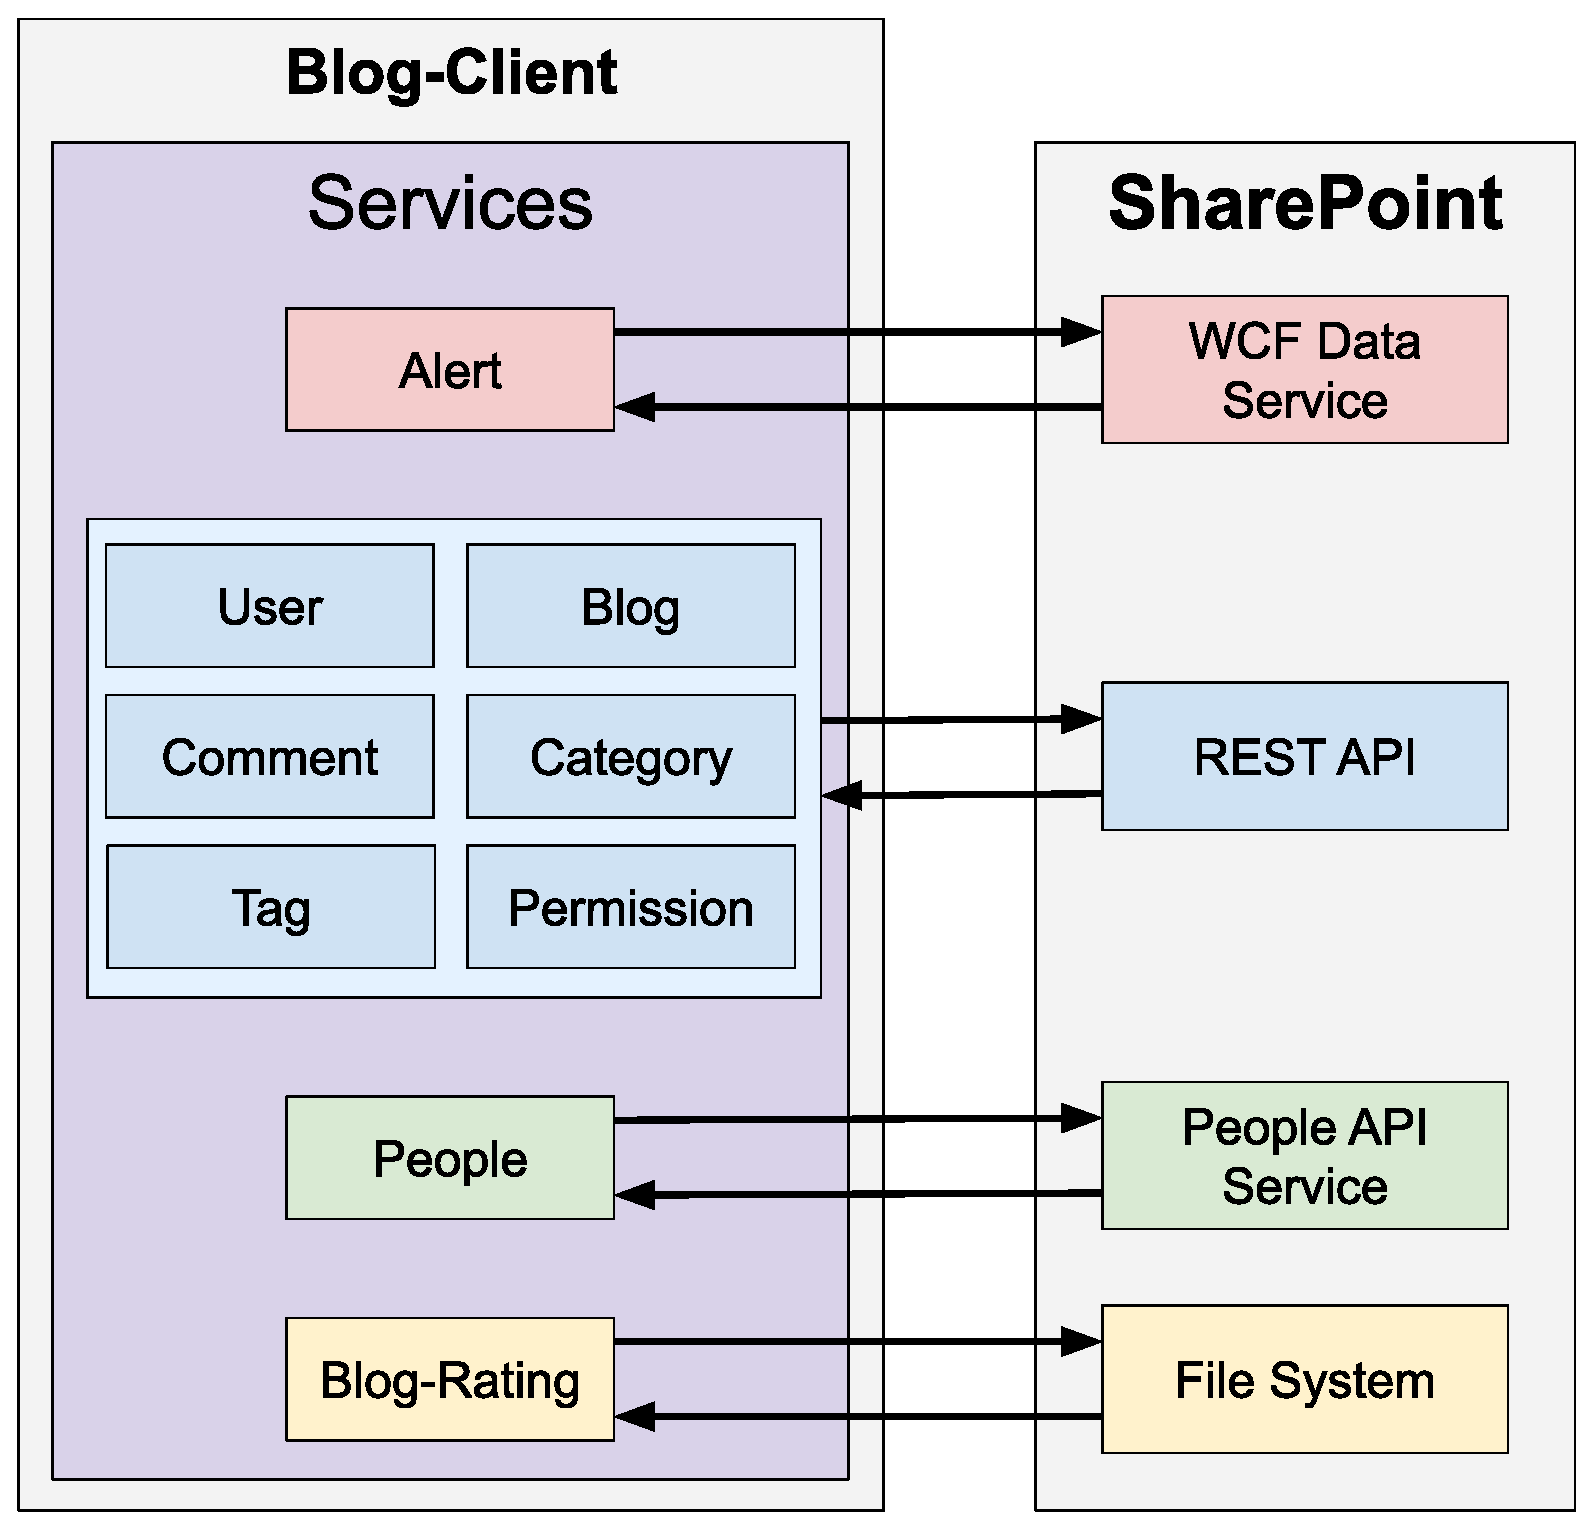
\includegraphics[width=0.85\linewidth]{PICs/communication_sharepoint_services.eps}
\caption{The different interfaces required to get all the data from SharePoint}\label{Fig7}
\end{figure}

Six of the nine services were able to request the required data from the SharePoint REST API. The SharePoint REST API expects a request corresponding to the OData (Open Data) protocol. This request is then processed by the "client.svc" web service of the SharePoint and depending on what is specified in the response type of the request, either a response in Atom or JSON format will be returned. In addition to the SharePoint REST API, alternatives such as the Client-Side Object Model (CSOM) API \cite{CSOM} or JavaScript Object Model (JSOM) \cite{JSOM} can be used to query data. However, Microsoft recommends using the SharePoint REST API for client-side customizations, but as long as the REST API offers not all functionality, any alternative is still supported.
\\[\baselineskip]
To keep assembling the queries for the REST API as simple as possible, the fluent JavaScript API, PnPJS \cite{Pnpjs}, developed by Microsoft was utilized. This library allows queries to be generated by chaining methods and then sent to the REST API without having to additionally use an HTTP client. If possible, every service was implemented using this technology.
\\[\baselineskip]
The required functionality of the alert service was not supported by the SharePoint REST API and therefore not by PnPJS, which is why an alternative decision was made to implement a WCF Data Service, as shown in Figure \ref{Fig7}. Since a WCF Data Service also uses the OData protocol, this service could be seen as a custom extension of the SharePoint REST API. For querying data, the Angular HTTP client was injected into the service.
\\[\baselineskip]
The people service had the same problems as the alert service. However, no separate WCF data service had to be developed here because no data was created but only requested. Therefore, employing an HTTP client was enough to communicate with the SharePoint People API service, as illustrated in Figure \ref{Fig7}. However, another limitation occurred when querying data with an Angular HTTP client the request was not accepted unless an authentication token was included in the request. This token could only be obtained by requesting authentication only. However, this did not have to be implemented if the SharePoint HTTP client was employed since it already does the authentication by itself.
\\[\baselineskip]
The rating feature of a blog post should be able to be switchable between the average number of stars and the number of likes given by users. Furthermore, when hovering over the rating, the names of people who have already rated the blog post should be displayed. Finally, hovering over a person should display a window that includes the person's Outlook (Microsoft Corporation, Redmond WA) profile. A request from the customer was that these features are always up to date without reloading the page. Since the SharePoint REST API did not provide any methods for this and the implementation with a WCF Data Service was based on executing scripts in the SharePoint file system, the blog-rating service was implemented using the SharePoint JavaScript Class Library \cite{SpJavaScriptClassLibrary}. As a result, using the SOD (Script On Demand) class \cite{SpSod}, the respective scripts used for the above functionalities could be registered and executed when changing the state of the rating.
\\[\baselineskip]
Before a service returned the response, the data residing on service entities was mapped to an entity convenient to the components. As a result future changes to the services only affect the service entities and the mapping.


\subsection{Styles}
Cascading Style Sheets (CSS) is the standard language used to describe the design of an HTML structure. Over 90\% of web developers use CSS, although some familiar programming constructs such as variables are not supported. Since it often happens that a customer does not like some aspects of the design, such as the color of icons, this often results in an effort that was not entirely planned. This effort increases especially if more CSS code is present than really needed, no structure is defined in the CSS files, and one CSS class affects several elements of the website. In order to keep this effort as low as possible, technologies such as Sass (Syntactically Awesome Style Sheets) \cite{Sass} and Bootstrap \cite{Bootstrap} were included, and the methodology BEM (Block Element Modifier) \cite{BEM} was utilized in defining the structure of the styles.
\\[\baselineskip]
In order to create a responsive website, Bootstrap's Container \cite{BootstrapContainer} and Grid \cite{BootstrapGrid} CSS classes were utilized. Thereby CSS classes that would have to take care of the layout did not have to be developed, leaving the Sassy Cascading Style Sheet (SCSS) files clearer.
\\[\baselineskip]
\begin{figure}[!htbp]
\centering
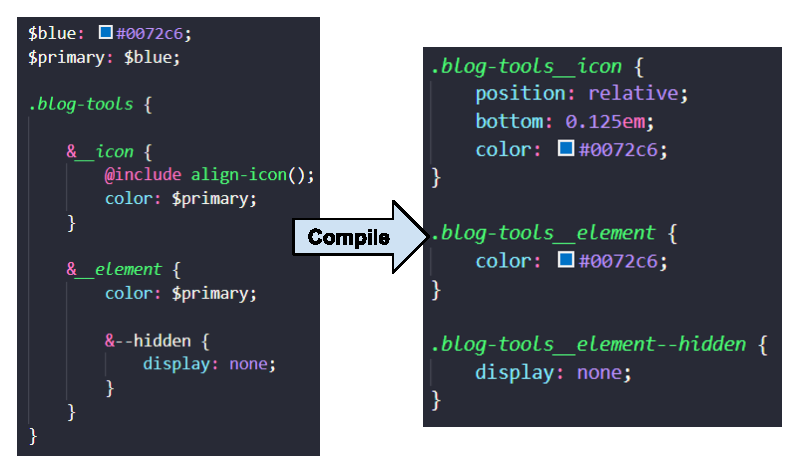
\includegraphics[width=0.75\linewidth]{PICs/sass_parent-selector_mixins_variables.eps}
\caption{An SCSS file (left) and the resulting CSS file (right) after compilation.}\label{FigSass}
\end{figure}

Sass is a CSS preprocessor, which provides the ability to manage variables, mixins, nesting, and a lot more to define the design of a component. The creators of Sass describe it as "CSS with superpowers" \cite{Sass}. The written code resides in so-called SCSS files and is transformed from the preprocessor compiler to plain CSS as the application builds, as shown in Figure \ref{FigSass} \cite[p.~168]{CSSPreproc}. For the preprocessor to recognize a variable, the name of the variable must start with a "\$" \cite[p.~169]{CSSPreproc} \cite{SassVariables}. Variables were mainly employed for colors because they were required in several places and were changed most frequently during the development. When creating a variable for colors, it was essential to initialize a second variable with the first as its value, as shown in Figure \ref{FigSass} in the SCSS code. Because then the name of the variable only had to be adjusted in the top of the SCSS file where all variables had to be declared. 
\\[\baselineskip]
Furthermore, a Mixin was defined, which was applied to all icon CSS classes so that the size and orientation of them remained the same. How to integrate a mixin into an SCSS file is shown by the "align-icon" mixin in Figure \ref{FigSass} in the SCSS code \cite{SassMixin}. A mixin can specify a group of styles, which can then be utilized throughout the project by including the mixin into the respective CSS class \cite[p.~170]{CSSPreproc} \cite{SassMixin}. In order not to unnecessarily compile a mixin, which is not included in any SCSS class, all mixins were defined in a partial SCSS file. Partial SCSS files can be identified by an underscore at the beginning of the filename \cite{SassPartial}.
\\[\baselineskip]
The nesting feature and the parent selector "\&" allowed to create a hierarchical structure of the SCSS files, which is similar to the HTML structure \cite[p.~169-170]{CSSPreproc} \cite{SassParent} \cite{SassNesting}. This structure was constructed by interlacing multiple SCSS classes together, avoiding some boilerplate code in the process \cite{SassNesting}. Through the parent selector, which references the outer selector, even more boilerplate code was circumvented \cite{SassParent}. As a result, as in Figure \ref{FigSass}, the "\&\_\_ icon" class is compiled into the "blog-tools\_\_icon" class.
\\[\baselineskip]
In order for the structure of the SCSS files to be implemented uniformly, BEM was adopted as a naming convention. The rules that came with it were the following: 
\begin{itemize}
\item Entities that are meaningful by themselves, such as the "div" element that houses the blog tools, are considered as a block. This "div" elements would, therefore, be given the CSS class "blog-tools" \cite{BEMNaming}.
\item Entities that do not make sense on their own are called elements, hence the elements of the blog tool got the class "blog-tools\_\_element" \cite{BEMNaming}.
\item A CSS class that causes a change in the appearance, behavior, or state of an entity is called a modifier. In Figure \ref{FigSass}, the class "blog-tools\_\_element-hidden" describes a modifier that defines the change in visibility of an element of class "blog-tools\_\_element" \cite{BEMNaming}.
\end{itemize}


\section{Reactive Programming}
This section is intended to clarify the development process associated with using Reactive Programming in Angular.
\\[\baselineskip]
For this purpose, the libraries and tools employed for this project are outlined and shown how they contributed to a more pleasant and faster development phase. Furthermore, the steps employed for adding new features to the structure defined by Redux and NgRx will be showcased. The last chapter explains the procedure of creating unit tests for the project and what methods can be used to develop unit tests for reducer and effects.

\subsection{Libraries \& Development Tools}
rxjs,
\\[\baselineskip]
\begin{figure}[!htbp]
\centering
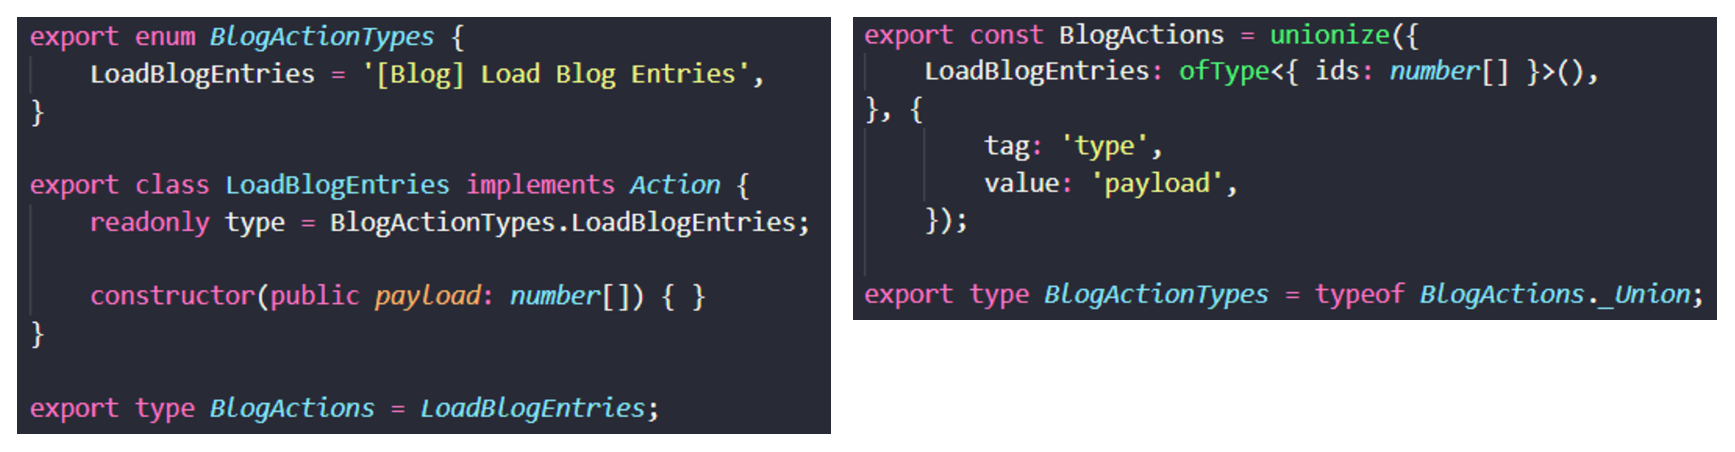
\includegraphics[width=1\linewidth]{PICs/without_and_with_unionize_actions.eps}
\caption{"LoadBlogEntriesAction" implemented without (left) and with the use of the methods "unionize" and "ofType" from the TypeScript library Unionize \cite{Unionize} (right).}\label{Fig4}
\end{figure}
easier use of the redux pattern through Unionize \cite{Unionize} (removing some boilerplate code for writing actions (unionize, ofType), reducers (Action.match) and effects(Actions.is.SpecificAction)).
\\[\baselineskip]
\begin{figure}[!htbp]
\centering
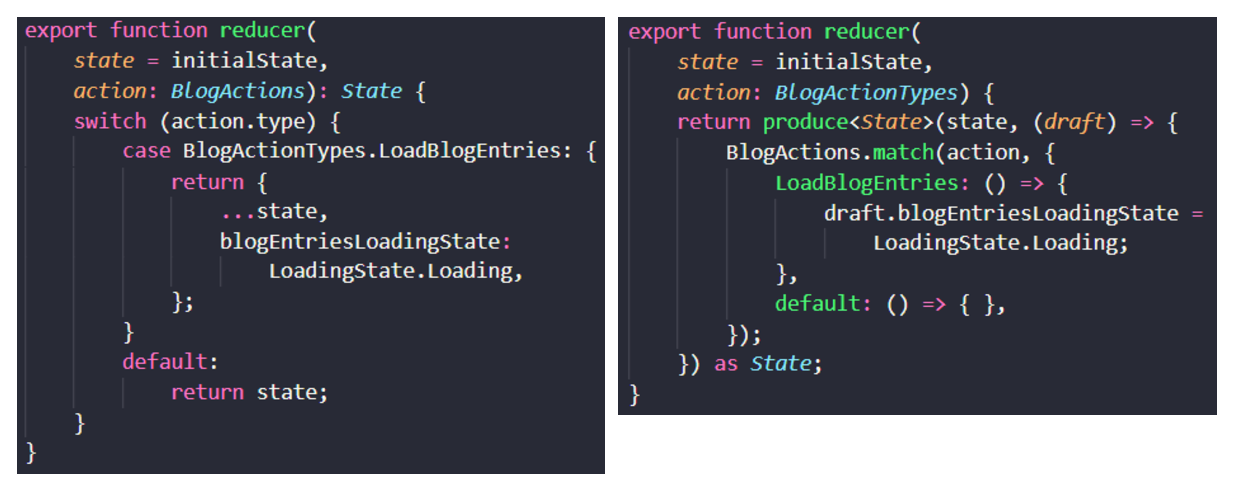
\includegraphics[width=1\linewidth]{PICs/with_and_without_immer_unionize_reducer.eps}
\caption{"BlogReducer" implemented without (left) and with the use of the methods "produce" and "match" from the JavaScript library Immer \cite{Immer} and the TypeScript library Unionize \cite{Unionize} (right).}\label{Fig5}
\end{figure}
Immer \cite{Immer} (removing some boilerplate code for writing reducers (produce)).
more features for reactive programming, Redux DevTools \cite{ReduxDevTools} as browser extension allowing time-travel debugging by importing the store devtools of ngrx into the AppModule.

\subsection{Adding a new Feature}
Whenever a new feature had to be integrated into the application, the question arose whether the local state would be sufficient for the functionality that this component should provide. Although it was often sufficient to manage a local state, there were occasionally good reasons why the store should be utilized. One of these was when the new feature needed to query data from SharePoint for which no container or service already existed. If a local state were still managed, the component would have to speak directly to the service. This would then lead to the fact that when changes to the SharePoint or changes to the requirements happened not just the service but also the component would have to be adjusted. Besides, this approach would speak against the agreed software architecture, which was discussed in Chapter 3.4. This problem was avoided by decapsulating the component from the service using the Redux pattern, supported by NgRx. In order to use this pattern, a structure as shown in Figure \ref{Fig6} had to be established.
\\[\baselineskip]
\begin{figure}[!htbp]
\centering
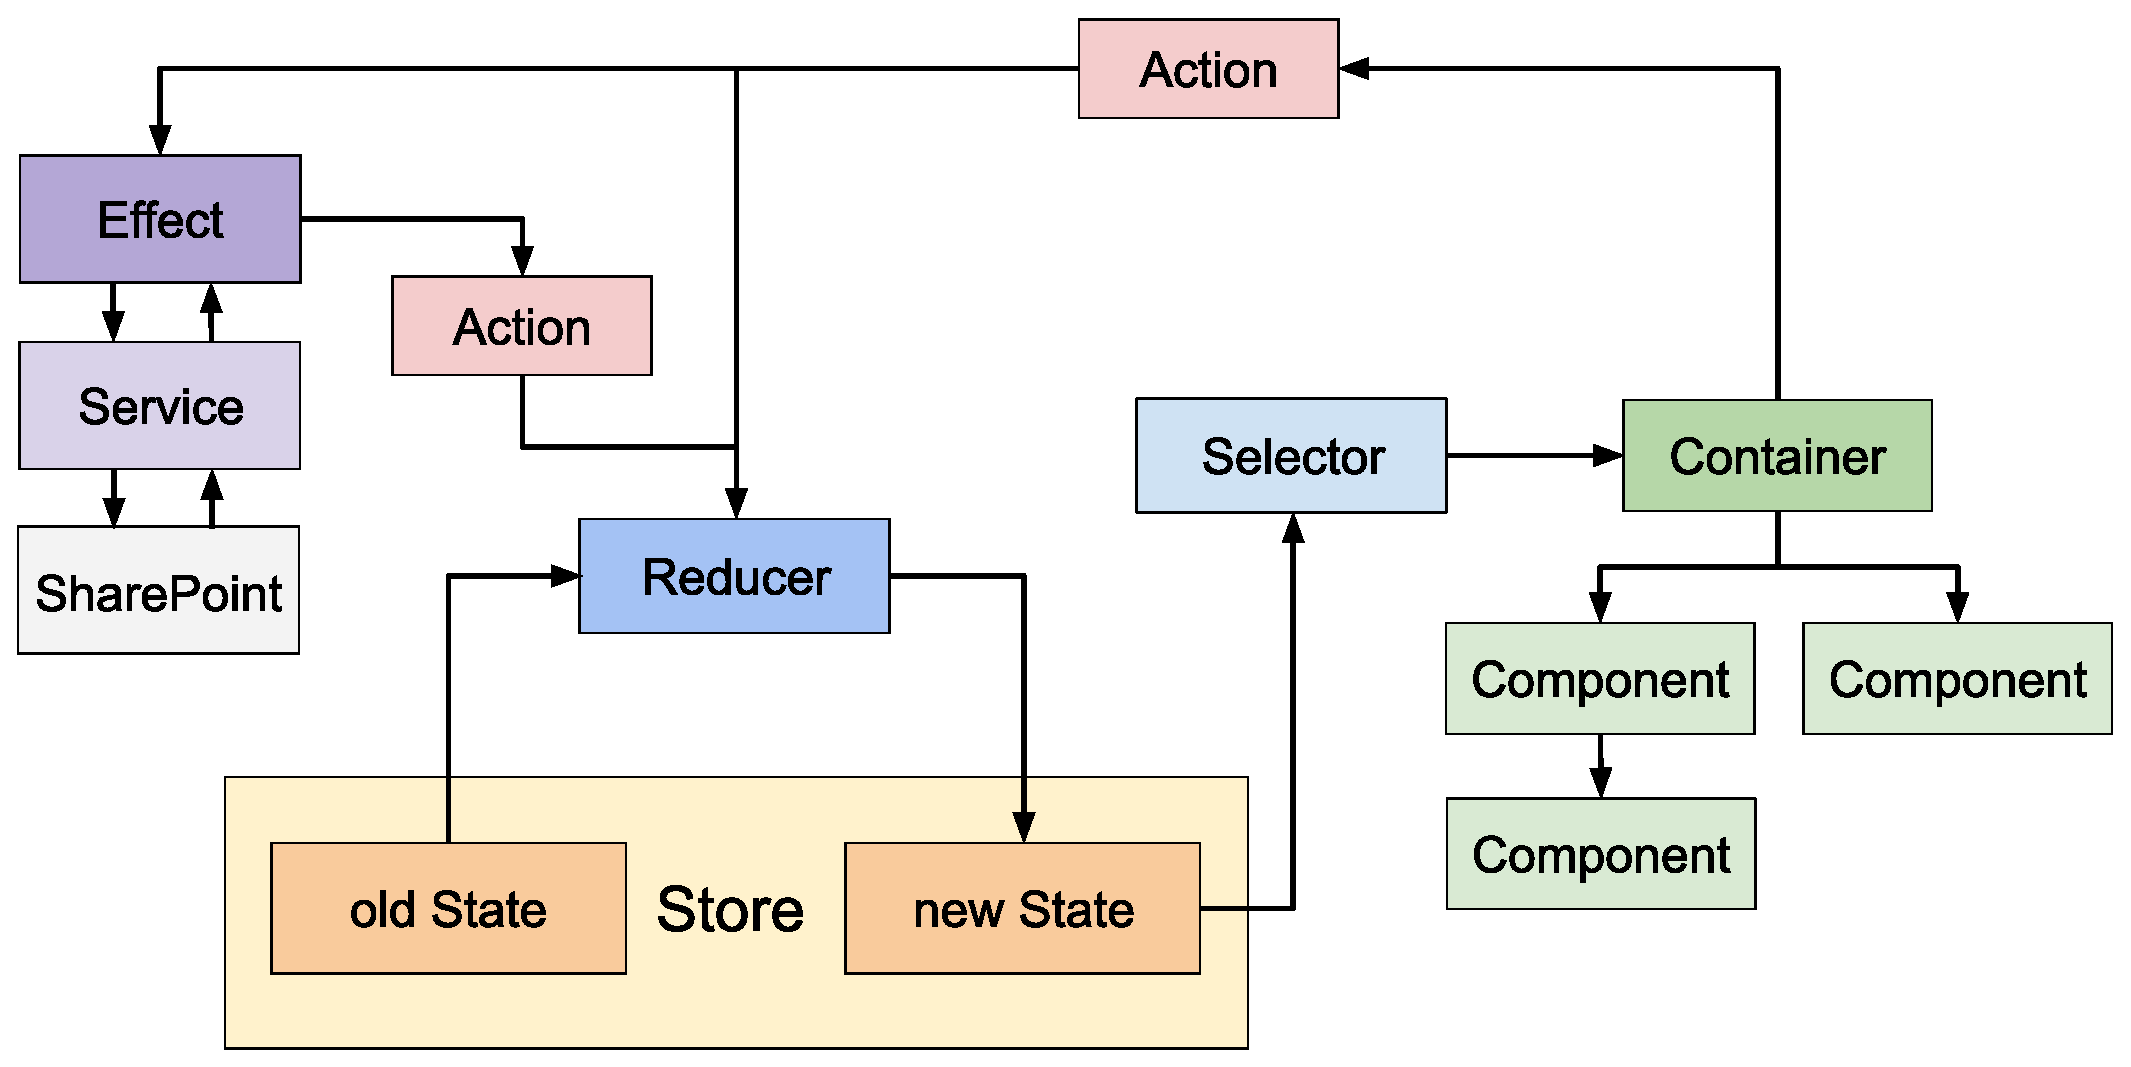
\includegraphics[width=0.85\linewidth]{PICs/ngrx_redux_structure.eps}
\caption{The Redux pattern in conjunction with NgRx}\label{Fig6}
\end{figure}
To clarify the structure of Figure \ref{Fig6} and the process behind adding a new feature, the implementation of the blog tools feature is described as an example. This feature consists of five links, as shown in Figure \ref{FigBlogDetail} on the left, that redirect to the blog management tools of the SharePoint. The reason why a local state should not be utilized here is that depending on the user's permissions different links have to be displayed. The following points describe what steps to take to integrate the blog tools feature into the Redux and NgRx structure:
\begin{itemize}
\item Create a container or component: At the beginning, the decision has to be made as to whether a suitable container already exists in which the blog tools component can be accommodated. Since the blog tools should be placed in the blog list page and the blog detail page both containers would have to implement the same code so that the blog tools component gets the data it needs. In order to implement requesting the data from the store only once, the blog tools feature has become a separate container.
\item Defining actions: Actions have to be implemented in order to allow the blog tools to communicate with the store. Since the blog tools are part of the blog module, the new actions have to be added to the "BlogActionTypes". Since user permissions have to be requested from SharePoint, three actions have to be defined, one for triggering the query, one for SharePoint's successful response, and one for SharePoint's failed response. In this case, these are the "LoadBlogToolsPermissions", "LoadBlogToolsPermissionsSuccess" and "LoadBlogToolsPermissionsFail". Since the user permissions do not have to be changed, the payload of the "LoadBlogToolsPermissions" action should stay empty. The success action should define an object for their payload that can be utilized in the blog tools component for creating the view. In this case, the object consisted of five boolean values, which determined if a link should be displayed or not. The fail action should return the payload type "any" since in the effect the error objects will be wrapped with the fail action before emitting.
\item Adapt state: For a reducer to be defined, the state must first be modified. In the state of the blog reducer, two properties have to be created. One holds the data returning from the effect, e.g. "blogToolsPermissions" and the other takes care of the loading state of the data, e.g. "BlogToolsPermissionLoadingState". The loading state simulates the loading of the data. As long as the loading state is set to "loading", a loading screen can be displayed, if the loading state changes to "loaded" or "failed", the application should react accordingly. Now the initial state has to be extended by the "blogToolsPermission" and the "blogToolsPermissionLoadingState" properties. The blog tools permission object is set to "null" and the loading state to "indeterminate".
\item Add Reducer: Since one reducer takes care of one action, three reducers have to be created. The reducer listening to the load-blog-tools-permissions action sets the blog-tools-permission-loading-state property of the state to "loading". The reducer listening for the success action sets the loading state to "loaded" and populates the blog-tools-permission object with data. The reducer, who listens for the error action, sets the loading state to "failed".
\item Create selector: In order for the container to be able to select the data, a selector must be defined for the blog-tools-permissions and the blog-tools-permissions-loading-state properties. For this purpose, two new variables are added to the blog selector file and defined by employing the "createSelector" method of NgRx. Thereby the store knows for which property of the state the respective variable is responsible.
\item Create service and mapping: In order that the effect does not have to query the required data itself, a service should be built which provides methods to communicate with SharePoint. Since only the user permissions need to be requested for the blog tools feature, the service should only provide a GET method that queries the required data from SharePoint. Before the data is returned, a mapping to a blog-tools-permission object should take place.
\item Define effect: In order for the user permission service to be triggered by actions, an effect must be defined by extending the blog effect class with a new property. This property must be marked with the "@Effect" decorator of NgRx to recognize it as an effect. In order for the effect to know to which action it should respond to, all actions that pop up should be checked if any of them matches the respective action. Depending on what needs to be implemented, it may happen that an effect still has to select data from the store or even request data form other services, but this is not the case with this effect. Therefore, the service is called immediately after filtering the appropriate action. Depending on whether the received response matches the expected data, a success or an error action will be emitted.
\end{itemize}

\subsection{Unit Testing}
In order to be able to react in the best possible way concerning changes in the requirements or additional orders of features, an attempt was made to cover most lines of code which concern the logic of the application with unit tests. Since refactoring already existing features or adding new features often causes bugs to creep into the application, a process similar to Test Driven Development (TDD) \cite{TDD} was adopted.
\\[\baselineskip]
This process demanded from the developer to create a unit test for the specific reducer at the exact time when the developer realized the component could only provide the functionality with a state managed inside of the store. If a service was responsible for obtaining the data and therefore an effect had to be implemented, a unit test for the effect had to be built as well. This process also made the learning curve of the Redux pattern flatter, or at least faster to learn, because forgetting one of the steps described in the previous chapter 3.5.2, lead to failing at least one unit test. This meant that one was constantly reminded of the Redux pattern. 
\\[\baselineskip]
Since the unit test is also created before the implementation of the reducer or the effect, the test thus always fails as long as no further implementation takes place. If one had to adhere strictly to TDD after the actions have been defined, the action should immediately be implemented in the unit test. However, the development team agreed that the unit test should not be fully implemented until after the state was established or extended, and the logic of the reducer was implemented.
\\[\baselineskip]
To make working with unit tests as comfortable as possible, the configuration of the Karma test runner \cite{Karma} generated by the Angular CLI was extended. The default test results reporter was removed, and the Karma-Mocha reporter \cite{KarmaMocha} and the Karma-Jasmine-Html \cite{KarmaJasmineHTML} reporter were included. The Karma-Mocha reporter explicitly printed out each unit test in the console in comparison to the default reporter, which only outputs the total number of successful test results. Another advantage is that if an error occurs during testing, the Karma-Mocha reporter still prints all the test results. Thus, where the problem is, can be narrowed down not only by the error message but also by the successful unit tests. Besides, the output is structured more clearly. The Karma-Jasmine-Html reporter was included for the same reasons, so each developer could decide for themselves which one to employ.
\\[\baselineskip]
Jasmine \cite{Jasmine} was utilized as the testing framework, as the team had already gained the most experience with it and it was possible to test effects when including another library. The format used to structure the unit tests was Given-When-Then \cite{GivenWhenThen}.
\\[\baselineskip]
For the unit tests of the reducer, an interface was created, which describes a test case. For each test case, the action, the name of the action, the name of the test, the current state, and the expected state had to be specified. Through this interface, it was possible to define all test cases as objects and to collect them in a list. Since the task of a reducer is only to change the state, a single unit test had to be written for all reducers, which saved much boilerplate code. Then, for each entry in the list, the single unit test, which checked whether the expected change of the state took place, was executed. 
\\[\baselineskip]
To test the effects with unit tests, a way had to be found how they could be called in a test. Effects need an action to trigger them and a service to get the data so that the effect can decide if a success action or fail action should be emitted. Hence, the first step was to create a setup method. All actions for the unit tests were made available utilizing the "provideMockActions" method of NgRx. Through the "TestBed" API of Angular, the effects and the services could be provided.
\\[\baselineskip]
A solution still had to be found to emit an action to trigger an effect. However, the developers of ReactiveX had already dealt with this topic and published a guide \cite{TestingMarbles}. The solution is to describe the mock observables through ASCII marble diagrams. An ASCII marble diagram might look like this: '-a-b-(cd)-|'. Each '-' sign stands for one frame of virtual time, the letters (could also be numbers) indicate that a value is emitted at this point, the brackets describe a point in time at which several values are emitted simultaneously, and the '|' sign means that the observable has been completed \cite{TestingMarblesSyntax}. An observable created with an ASCII marble diagram does not have to have a '|' character at the end. Doing so results in the observable never calling its "complete" method. A blank space inside of an ASCII marble diagram will be ignored and should be adopted to vertically align the statement \cite{TestingMarblesExamples} \cite{TestingMarblesSyntax}.
\\[\baselineskip]
An observable can also be created with an ASCII marble diagram, which only emits the next value after a long time. For example, the ASCII marble diagram 'a 9ms b' creates an observable which emits the value 'a' on frame 0 and the value 'b' on frame 10. When defining time units, it is necessary to add blank spaces between the characters since the ASCII marble diagram 'a9msb' would create an observable, which emits one frame after the other the values of 'a', '9', 'm', 's' and 'b'. In addition to ms (milliseconds), s (seconds) and m (minutes) are available as definable time units \cite{TestingMarblesTime}.
\\[\baselineskip]
ASCII marble diagrams also support "hot" and "cold" observables. In order for a "hot" observable to behave as if an observer subscribed to the observable, the '\string^' character can be used to identify the point in time at which the new observer has subscribed. A "hot" observable created by an ASCII marble diagram could look like this: '- a - \string^ - b'. A new Observer would, therefore, receive the value of 'b' but not the value of 'a' \cite{TestingMarblesSyntax}. A subscription marble diagram makes it possible to test if an observer unsubscribes from an observable. An example of a subscription marble diagram would be '- \string^ - - - ! -'. Here again, the character '\string^' specifies the beginning of the subscription and the character '!' describes the point in time where an observer terminates the subscription \cite{TestingMarblesSubscribe}. This also allows asserting whether an observer received the values that the observable emitted while the subscription was still active. For example, with an observable 'a b c' and a subscription marble diagram '- \string ^ - !', an observer would only get the value of 'b' because the value of 'a' was emitted before the observer was subscribed and the value of 'c' could no longer be received because at the same moment the subscription was terminated \cite{TestingMarblesSubExamples} \cite{TestingMarblesSubscribe}.
\\[\baselineskip]
By incorporating the Jasmine-Marbles library \cite{TestingMarbles}, which provides the functionality described above, the actions could be emitted through an observable to trigger an effect. Also, the respective service had to be mocked through the "spyOn" method of jasmine.
\\[\baselineskip]
Furthermore, a "cold" observable was created to define the expected value of the effect. Since the effects always emitted only either a success action or a fail action, the expected observable was defined with the ASCII marble diagram '--s'. The value of 's' was either the success action or the fail action. In order to finally compare the expected observable with the respective effect, the methods "expect(effect).toBeObservable(expected)" were employed.

\clearpage


\chapter{Discussion}
The following sections address the implementation difficulties, discuss the methods used to develop the project, and present the final product.

\section{Development}
The development time of this project was initially almost equated with the expansion of the old project. However, instead of the estimated 358 hours, a total of 434 hours were worked on the Angular project. This 76-hour difference may be due to the initial steep learning curve of reactive programming, and Redux combined with Angular. Since 2 of 3 developers had no experience with reactive programming or the Redux pattern before the project.
\\[\baselineskip]
In addition, the implementation of the services was underestimated. One of the reasons for this was because the developer team initially thought the SharePoint REST API supported fetching all the data stored in SharePoint. However, as described in chapter 3.4.2, several solutions had to be developed to get all the required data from SharePoint. Especially, a lot of time was lost in developing the alert WCF Data Services. The task was estimated to take 13 hours but ended up taking 27.66 hours.
\\[\baselineskip]
The Redux pattern in combination with NgRx initially caused confusion because the different components (action, reducer, state, selector, effect, service) are almost too encapsulated for a beginner to keep track. As a result, developing the first features often consisted of jumping from one file to another and back again. Due to the daily stand-ups and the CI, this problem was detected early, and therefore processes were defined for the implementation of the Redux and NgRx structure, see chapters 3.5.2 and 3.5.3.
\\[\baselineskip]
Nevertheless, the first days were spent mainly with learning how to develop with reactive programming efficiently. However, above all, there were significant advantages in using this pattern and the module-based layout of the project. By encapsulating the software components, new features could be added without having to refactor a significant part of existing software components. As described in chapter 3.5.2, the actions, reducers, states, selectors, effects, and services have to be extended for a new feature but only if the logic of the new feature requires a global state.
\\[\baselineskip]
Some minor changes have to occur in the HTML file of the parent component because the new feature has to be integrated. Also, changes to the SCSS file could be likely, but through the use of BEM, most of the work would consist of extending the file instead. 
\\[\baselineskip]
Real changes to already existing components will only have to happen if an already existing feature has to be altered or extended. Opposed to the old SharePoint application, where care had to be taken to ensure that an injected JavaScript code does not affect the site to be extended and a manager class manages more than it should, thereby influencing other software components, extending the Angular application is much more comfortable and far less time-consuming.
\\[\baselineskip]
Not much can be said about the maintenance work because so far no maintenance tasks have been incurred which affected the Angular application. Incurred maintenance work of this project has so far only affected configurations regarding SharePoint. However, if maintenance work has to be done for the Angular project, each member of the development team can now solve the problems compared to the old SharePoint solution where just one developer had enough knowledge to solve the arisen issues.
\\[\baselineskip]
However, to allow maintenance to be performed on the application by other development teams, at least one of these teams members should have knowledge of reactive programming in Angular with Redux. Since the steep learning curve of the applied methods in addition to understanding the entire software architecture would be too much effort, to resolve just one maintenance task. Nonetheless, if the necessary knowledge about the used technologies is available, then with Redux DevTools the application can be examined for sources of error. Also, the logs automatically generated by SharePoint can be viewed. If a bug is found, solving it would probably only affect the particular component where the bug is, because of how the communication between the software components was designed, as described in chapter 3.4. If on the other hand the issue is caused by a wrong implementation of the Redux and NgRx structure multiple components could be affected.
\\[\baselineskip]
The maintainability of the Angular application could be increased even further by installing server-side logging ourselves instead of using the automatic logging of SharePoint. This addition would lead to not having to require trusting the implementation of SharePoint's logging. Furthermore, depending on the implemented logging framework additional functionalities, like getting notified if errors are thrown or detailed error reports including the values of the last state before the error occurred, could be utilized (notifications if errors are thrown, e.g.).

\section{Results}
presenting finished solution
\begin{figure}[!htbp]
\centering
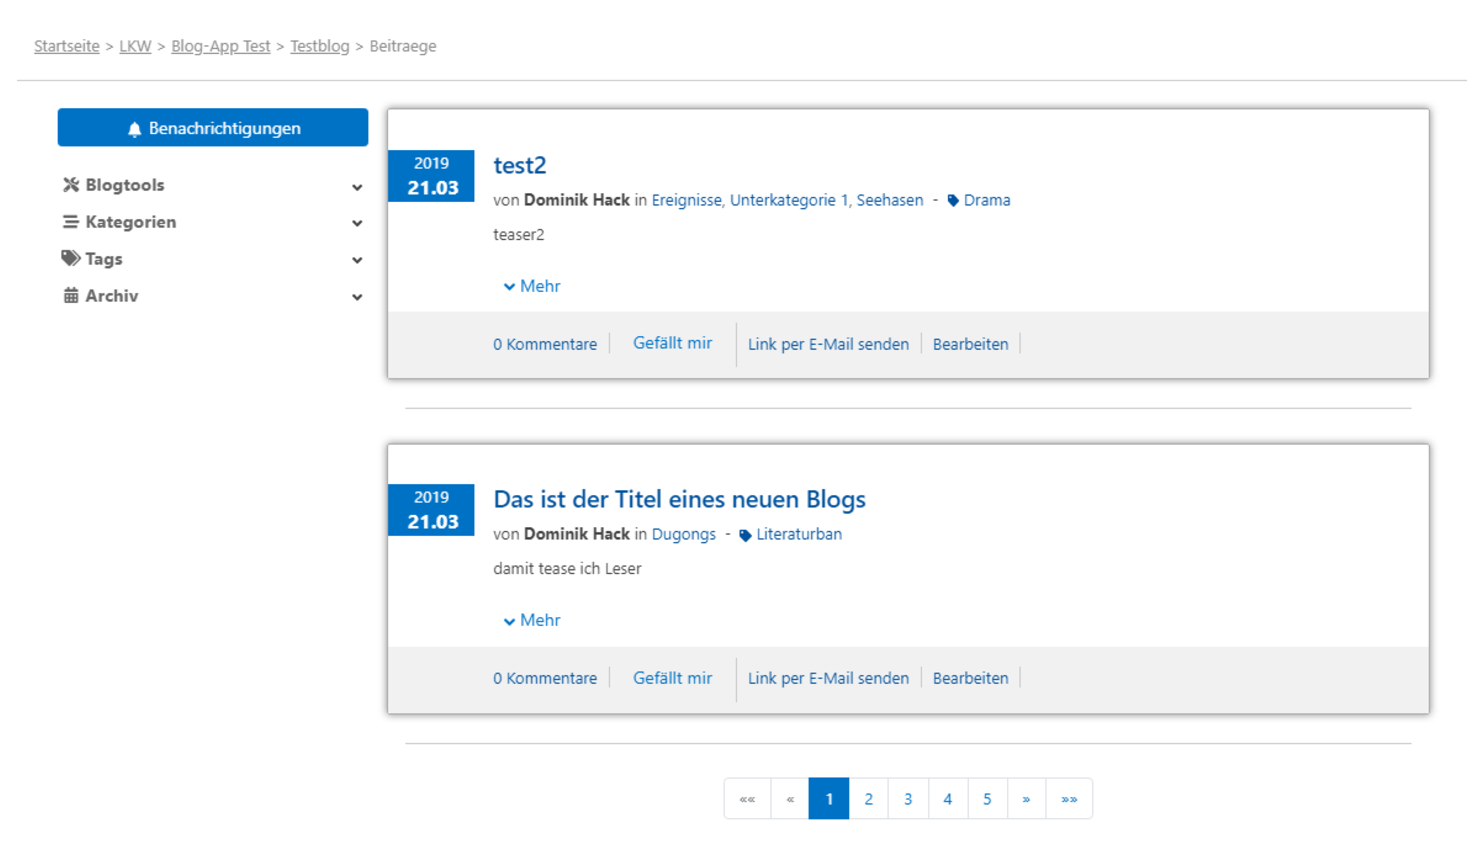
\includegraphics[width=1\linewidth]{PICs/blog_list_page.eps}
\caption{Blog List page}\label{FigBlogList}
\end{figure}
\begin{figure}[!htbp]
\centering
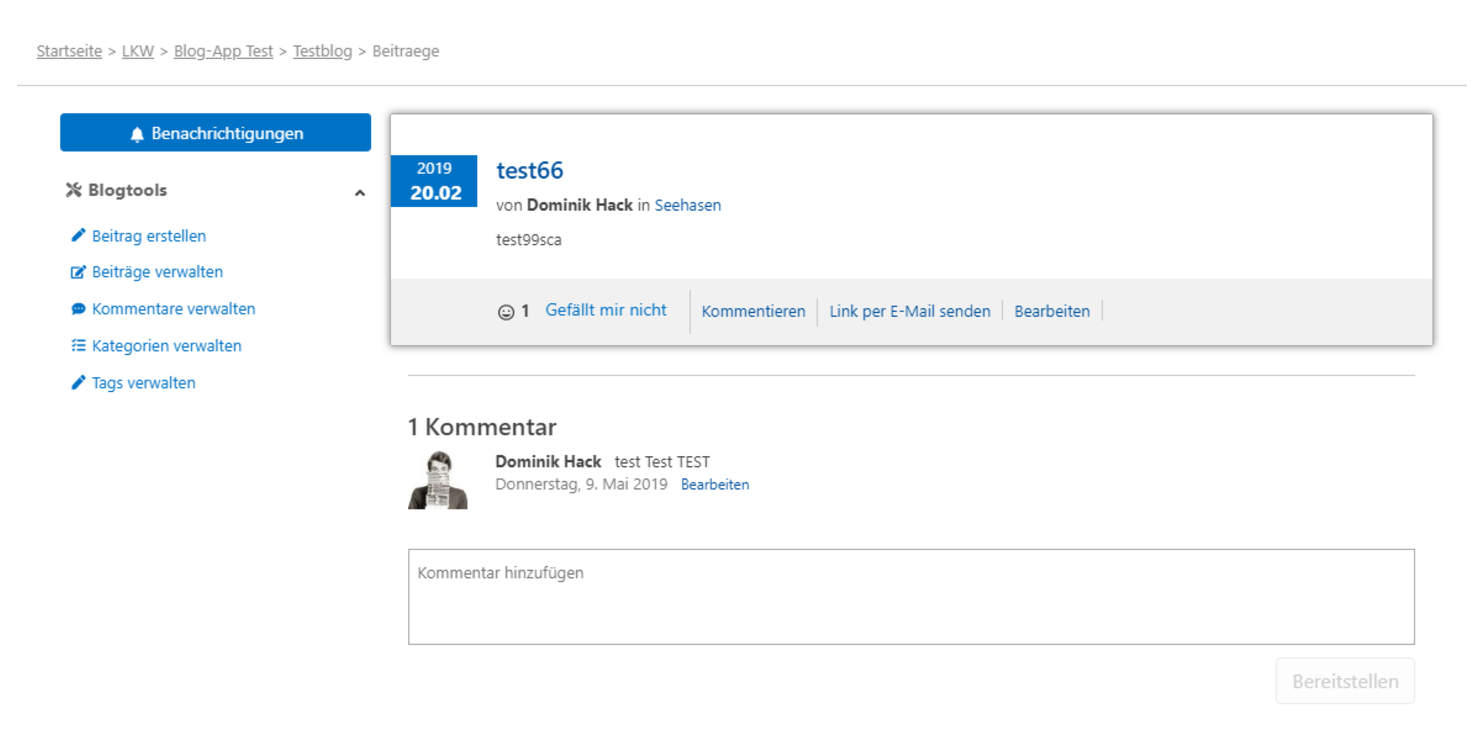
\includegraphics[width=1\linewidth]{PICs/blog_detail_page.eps}
\caption{Blog Detail page}\label{FigBlogDetail}
\end{figure}
\begin{figure}[!htbp]
\centering

\includegraphics[width=1\linewidth]{PICs/my_blog_alerts_page.eps}
\caption{My Blog Alerts page}\label{FigMyAlerts}
\end{figure}
\begin{figure}[!htbp]
\centering
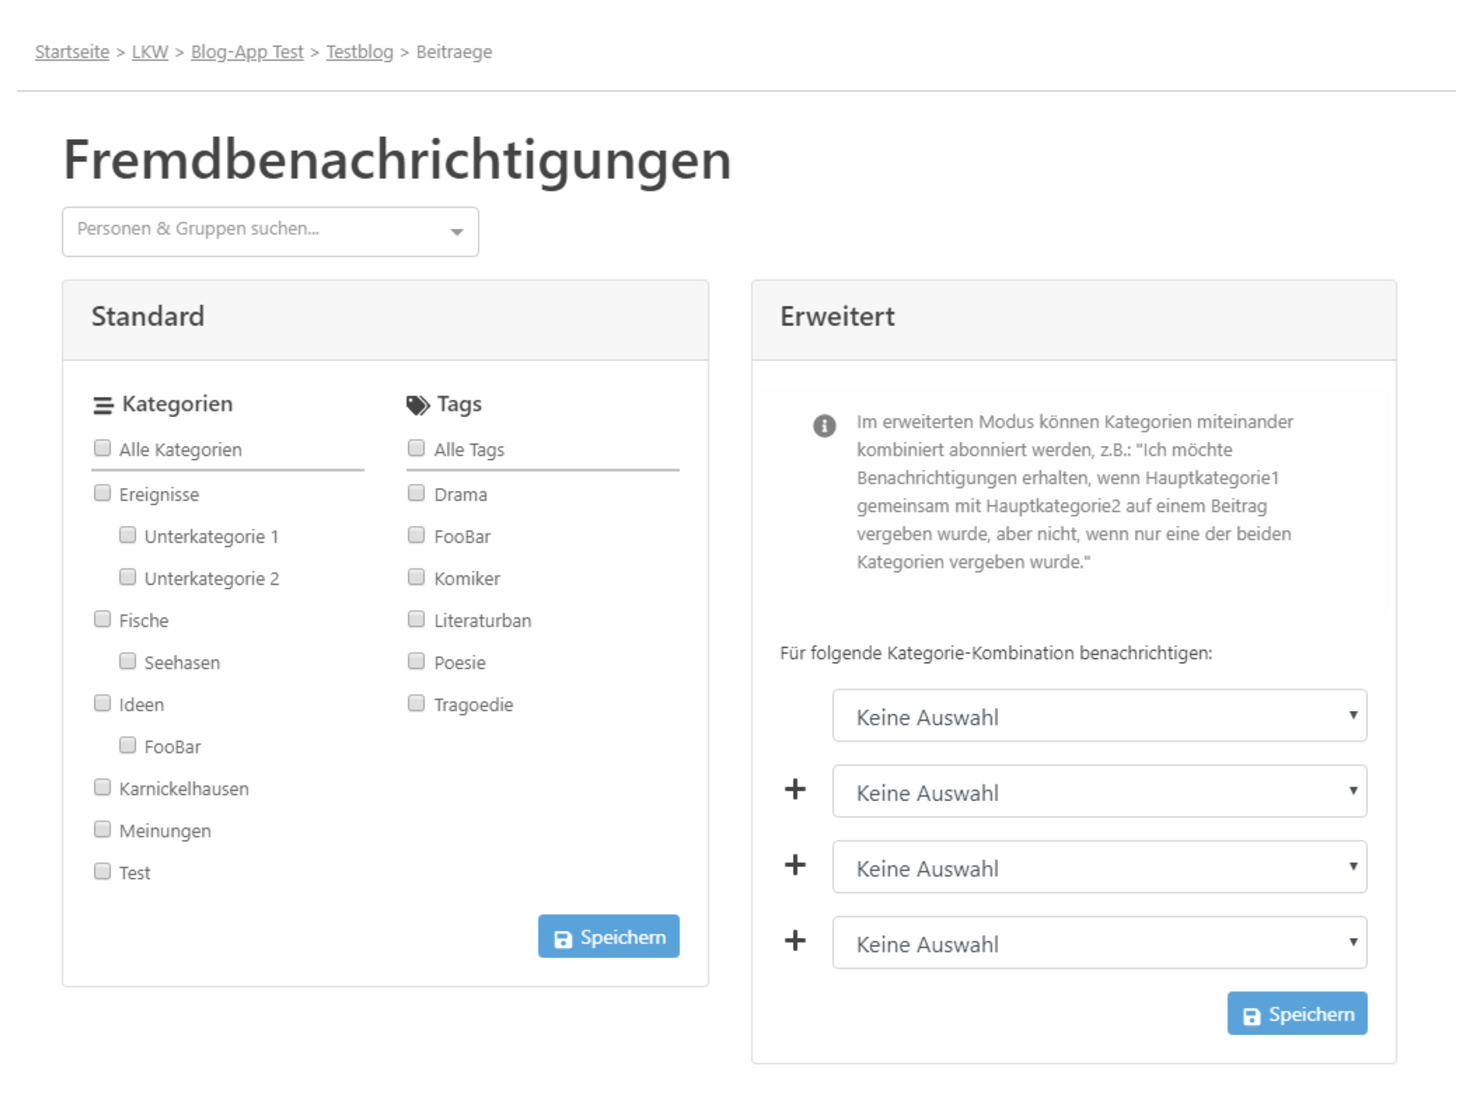
\includegraphics[width=1\linewidth]{PICs/mandatory_alerts.eps}
\caption{Mandatory Blog Alerts page}\label{FigMandatoryAlerts}
\end{figure}
\clearpage


\chapter{Conclusion \& Future Work}
Which changes have to be made in the project so that the application or already existing components can be extended in functionality?
Is the application more maintainable because it was implemented in a new project instead of the SharePoint project?

Zusammenfassend kann gesagt werden, dass eine Applikation entwickelt wurde, welche nur Abhängigkeiten vom SharePoint durch ihre Services hat. Würde in der Zukunft

herausgefunden wurde:
also extensibility, maintenance and encapsulation can more easily be improved when starting at zero,
Angular and RP works great together;
falls SharePoint für etwas anderes ersetzt werden soll müssten nur neue services für die neue API erstellt werden;

war ein Erfolg da schlussendlich Kunde zufrieden, Projekt konnte im erlaubten Zeitrahmen bleiben,
better for company to have knowledge in Angular than in Sharepoint 2013 (because more projects also use angular),

future work:
könnte versucht werden die blog features in das alte SharePoint Projekt einzubauen um herauszufinden ob die Entwicklungszeit kürzer oder länger dauert als das Angular Projekt,
ob ab wann das Redux pattern eingesetzt werden soll von der größe der Applikation abhängt und ob durch Redux zu viel Kapselung von Software Components entstand, somit das Projekt zu komplex wird um einem anderem Entwicklerteam Wartungstasks zu übergeben. Auf jeden Fall wäre das bisherige Problem, das wenige Wissen über SharePoint, was das bearbeiten von Wartungstasks betrifft kaum noch vorhanden, da nur die services eine Abhängigkeit zum SharePoint haben.


% Hier beginnen die Verzeichnisse.
\clearpage
\ifthenelse{\equal{\FHTWCitationType}{HARVARD}}{}{\bibliographystyle{gerabbrv}}
\bibliography{Literatur}
\clearpage

% Das Abbildungsverzeichnis
\listoffigures
\clearpage

\phantomsection
\addcontentsline{toc}{chapter}{\listacroname}
\chapter*{\listacroname}
\begin{acronym}[XXXXX]
    \acro{API}[API]{Application Programming Interface}
    \acro{ASCII}[ASCII]{American Standard Code for Information Interchange}
    \acro{BEM}[BEM]{Block Element Modifier}
    \acro{CLI}[CLI]{Command-Line Interface}
    \acro{CSS}[CSS]{Cascading Style Sheets}
    \acro{ECMA}[ECMA]{European Computer Manufacturers Association}
    \acro{GUI}[GUI]{Graphical User Interface}
    \acro{HTML}[HTML]{Hypertext Markup Language}
    \acro{HTTP}[HTTP]{Hypertext Transfer Protocol}
    \acro{REST}[REST]{Representational State Transfer}
    \acro{SASS}[SASS]{Syntactically Awesome Style Sheets}
    \acro{SCSS}[SCSS]{Sassy Cascading Style Sheets}
    \acro{SVG}[SVG]{Scaleable Vector Graphics}
    \acro{TDD}[TDD]{Test Driven Development}
    \acro{TFS}[TFS]{Team Foundation Server}
    \acro{XML}[XML]{Extensible Markup Language}
\end{acronym}

\end{document}}